% Tipo de documento
\documentclass[12pt,a4paper]{article}

% Pacotes
%\usepackage{showlabels}
\usepackage{latexsym}
\usepackage{amsfonts}
\usepackage{amsmath}
\usepackage{amscd}
\usepackage[brazil]{babel}
\usepackage[utf8]{inputenc}
\usepackage[pdftex]{graphicx} 

% Paginação
\textwidth 15.0cm                    % Largura
\textheight 23.0cm                   % Altura
\addtolength{\oddsidemargin}{-0.8cm}  % Margem esquerda (impar)
%\addtolength{\evensidemargin}{0.0cm} % Margem esquerda (par)
\addtolength{\topmargin}{-1.5cm}      % Margem superior

% Estilo dos parágrafos
\sloppy                              % Mais flexível
\setlength{\jot}{08pt}               % Distância entre linhas do eqnarray
\setlength{\parskip}{1ex}            % Distância entre parágrafos
\renewcommand{\baselinestretch}{1.0} % Distância entre linhas

% Contagem de equações por seção
\renewcommand{\theequation}{\thesection.\arabic{equation}}

% Contagem de figuras por seção
\renewcommand{\thefigure}{\thesection.\arabic{figure}}

% Contagem de tabelas por seção
\renewcommand{\thetable}{\thesection.\arabic{table}}

% Zerar as contagem em cada seção
\newcommand{\zerar}{\setcounter{equation}{0}\setcounter{figure}{0}\setcounter{table}{0}}

\DeclareMathOperator{\col}{col}
\DeclareMathOperator{\row}{row}

% Conjunto de números
\newcommand{\Z}{\mathbb{Z}}
\newcommand{\C}{\mathbb{C}}
\newcommand{\N}{\mathbb{N}}
\newcommand{\Q}{\mathbb{Q}}
\newcommand{\R}{\mathbb{R}}

%%%%%%%%%%%%%%%%%%%%%%%%%%%%%%%%%%%%%%%%%%%%%%%%%%%%%%%%%%%%%%%%%%%%%%%%%%%%%%%%%%%%%%%%%%%%%%%%%%%%

\begin{document}

\title{{\sc MAC0325 -- Otimização Combinatória} \\ 
\vspace{0.5cm} {\bf Escalonamento de Tarefas}}
\author{Daniel Augusto Cortez}
\date{\today}

\maketitle

\begin{abstract}
Relatório descrevendo a implementação e os resultados do projeto da disciplina MAC0325 - Otimização 
Combinatória, IME-USP 2013 (Escalonamento de Tarefas).
\end{abstract}

%%%%%%%%%%%%%%%%%%%%%%%%%%%%%%%%%%%%%%%%%%%%%%%%%%%%%%%%%%%%%%%%%%%%%%%%%%%%%%%%%%%%%%%%%%%%%%%%%%%%

\zerar
\section{Introdução}
\label{sec:intro}

Neste projeto, estuda-se o problema de se escalonar um determinado número de tarefas a um conjunto 
de máquinas idênticas e paralelas. Sejam $m$ o número de máquinas e $n$ o número de tarefas. Seja
$d_i$ a duração da tarefa $i$. Cada tarefa deve ser processada por exatamente uma máquina, sem 
interrupição. Objetiva-se minimizar o tempo máximo de ocupação das máquinas, o chamado {\it 
makespan}. O problema é denotado na literiarura~\cite{pinedo} por $Pm\,|\,|\,C_{max}$.

Seja $x_{ij} \in \{0, 1\}$ a variável de decisão que assume valor 1 se a tarefa $i$ for
atribuída a máquina $j$ e 0 caso contrário. O problema de minimização do {\it makespan} pode ser
formulado como
%
\begin{eqnarray} \label{eq:modelo}
\text{minimizar} && C_{max} \nonumber \\
\text{sujeito a} 
  && \sum_{i = 1}^{n} x_{ij} d_i \leq C_{max} \, , \;\; 1 \leq j \leq m \\
  && \sum_{j = 1}^{m} x_{ij} = 1 \, , \;\; 1 \leq i \leq n \, . \nonumber
\end{eqnarray}

$Pm\,|\,|\,C_{max}$ pode ser reduzido ao problema da 3-{\sc partição} sendo, portanto, de natureza 
$\mathcal{N}\mathcal{P}$-difícil. Um método heurístico simples para resolução aporoximada do 
problema de escalonamento foi desenvolvido por Graham na década de 60~\cite{graham}. O método, 
chamado de {\it List Scheduling Algorithm}, consiste na atribuição da próxima tarefa disponível a 
máquina de menor ocupação. É bem sabido~\cite{shmoys} que esse algoritimo resulta em uma 
$(2-1/m)$-aproximação

A heurística de Graham pode ser melhorada fazendo-se uso de uma estratégia gulosa. Primeiro 
ordena-se as tarefas em ordem decrescente no valor de suas durações. Em seguida, faz-se a atribuição
das tarefas nessa ordem a máquina de menor ocupação. Tal procedimento é conhecido pelo nome de {\it 
Longest Processing Time} (LPT) e resulta em uma $(4/3-1/3m)$-aproximação~\cite{shmoys}. Tal razão de 
aproximação é justa. De fato, considere uma instância com 4 máquinas e 9 tarefas, cujas durações são 
mostradas na tabela abaixa: 
%
\begin{equation*}
  \begin{tabular}{cccccccccc}
    \hline
    tarefas & 1 & 2 & 3 & 4 & 5 & 6 & 7 & 8 & 9 \\
    \hline
    $d_i$ & 7 & 7 & 6 & 6 & 5 & 5 & 4 & 4 & 4 \\
    \hline
  \end{tabular} 
\end{equation*}
%
Escalonando as tarefas de acordo com a heurística LPT resulta em um {\it makespan} igual a 15. 
Entretanto, para esse conjunto de tarefas um escalonamento ótimo pode ser encontrado com 
$C_{max} = 12$.

Neste projeto a heurística LPT é estudada empiricamente, comparando seus resultados com valores 
exatos obtidos pela resolução de (\ref{eq:modelo}) pelo otimizador CPLEX. Os resultados indicam, 
para as instâncias consideradas, que a heurística se comporta de forma muito melhor do que o 
esperado pela análise de pior caso.

%%%%%%%%%%%%%%%%%%%%%%%%%%%%%%%%%%%%%%%%%%%%%%%%%%%%%%%%%%%%%%%%%%%%%%%%%%%%%%%%%%%%%%%%%%%%%%%%%%%%

\zerar
\section{Implementação}

Na implementação realizada, uma classe básica \verb|Scheduler| foi projetada como interface para 
definir os métodos que as classes derivadas \verb|LptScheduler| e \verb|CplexScheduler| devem 
implementar. Tais métodos permitem a caracterização completa da solução gerada para uma instância do 
$Pm\,|\,|\,C_{max}$ passada, como, por exemplo, o valor do {\it makespan} resultante e a impressão
do escalonamento final. As classes \verb|LptScheduler| e \verb|CplexScheduler| implementam o 
procedimento de solução via heurística LPT e via otimzador CPLEX, respectivamente.

A comparação dos resultados é realizada através do cálculo da razão $LPT/OPT$ entre os valores de 
{\it makespan} obtidos pelas duas metodologias. É claro que uma mesma instância do problema deve ser
passada para as respectivas classes. Tal instância, na implementação, é representada por uma lista 
de máquinas e por uma lista de tarefas, podendo ser lida a partir de um arquivo de entrada 
padrão\footnote{Confira o arquivo README para obter informações sobre o arquivo de entrada e 
sobre as forma de utilização do programa.}, ou ainda gerada aleatoriamente.

A classe responsável pela geração das instância aleatórias é \verb|Generator|. Na instanciação do 
objeto associado, deve-se informa o número de máquinas e o número de tarefas pretendidas. O método 
\verb|generate(min, max)| gera as tarefas com durações inteiras {\it uniformemente distribuídas} no 
intervalo fechado [min, max]. O intuito da geração aleatória das instâncias é estudar o 
comportamento da heurística no caso {\bf médio}.

Na implementação da heurística LPT, as máquinas são inseridas em uma fila de prioridades ({\it 
heap}) que considera o valor de ocupação da máquina. Com isso, a operação de se obter a máquina de 
menor ocupação é realizada em $O(\log m)$, resultando em uma complexidade total para o algoritmo de 
$O(n \log m)$.

%%%%%%%%%%%%%%%%%%%%%%%%%%%%%%%%%%%%%%%%%%%%%%%%%%%%%%%%%%%%%%%%%%%%%%%%%%%%%%%%%%%%%%%%%%%%%%%%%%%%

\zerar
\section{Experimentos Numéricos}

A implementação realizada em C++ foi testada em uma máquina com processador 1.6 GHz Intel Core i5 
com 4GB de RAM, rodando o sistema operacional MacOS~10.7.2. 

Instâncias aleatórias foram geradas para diversos valores de $m$ e $n$, medindo-se 5 vezes o valor 
da razão $LPT/OPT$ entre os {\it makespans} das soluções encontradas. As durações das tarefas 
apresentam valores inteiros com distribuição uniforme no intervalo $[0, 1000]$. A 
Tabela~\ref{tab:medidas} mostra os resultados médios obtidos e a Figura~\ref{fig:medidas} traz a 
representação gráfica das médias com um intervalo de confiança de 67\% (um desvio-padrão).

As piores instâncias estudadas em termos de tempo de processamento, curiosamente, não ocorreram com
aquelas com maior número de variáveis. Na verdade, elas foram aquelas com $m = 16$ e $n = 40, 80$.
Nesses casos, o algoritmo {\it branch-and-bound} utilizado pelo CPLEX teve duração limitada a 3 
minutos, de forma que a solução apresentada não representa o valor ótimo, embora estivesse muito 
próxima dela (o processamento foi interrompido com gaps da ordem de 0.5\%-1.0\%).

\begin{table}[htbp]
  \begin{center}
    \begin{tabular}{|c|c|c|c|c|}
      \hline 
                & $m = 2$ & $m = 4$ & $m = 8$ & $m = 16$ \\
      \hline \hline 
      $n = 10$  & 1.00756 & 1.04135 & 1.00000 & 1.00000 \\ \hline
      $n = 20$  & 1.00198 & 1.01480 & 1.03009 & 1.00000 \\ \hline
      $n = 40$  & 1.00040 & 1.00550 & 1.02280 & 1.04043 \\ \hline
      $n = 80$  & 1.00030 & 1.00132 & 1.00560 & 1.02373 \\ \hline
      $n = 160$ & 1.00004 & 1.00031 & 1.00154 & 1.00514 \\ \hline
      $n = 320$ & 1.00002 & 1.00007 & 1.00028 & 1.00077 \\ \hline
      \end{tabular} 
      \caption{Valores médios da razão $LPT/OPT$ para diversas instâncias do problema 
      $Pm\,|\,|\,C_{max}$. As médias forma calculadas através de 5 instâncias
      geradas aleatoriamente para cada valor de $m$ e $n$.}
      \label{tab:medidas}
  \end{center}
\end{table}

\begin{figure}[htbp]
 \label{fig:medidas}
 \begin{center}
   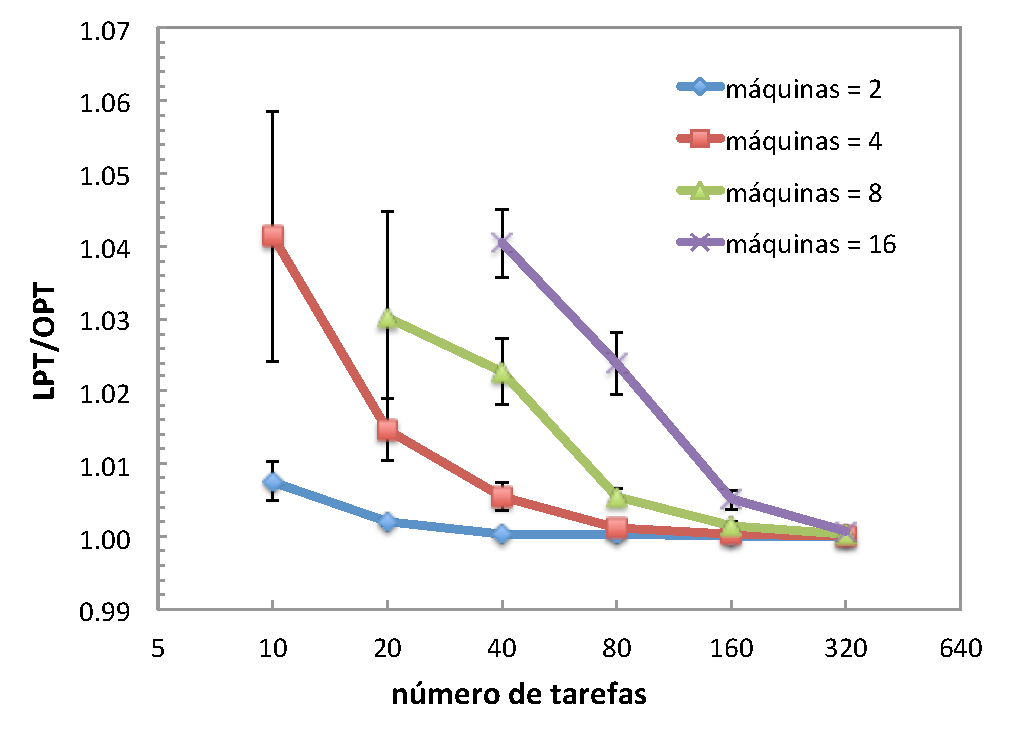
\includegraphics[scale=0.70]{../resultados/medidas.pdf}
   \caption{Representação gráfica dos valores médios da razão $LPT/OPT$ apresentados na 
   Tabela~\ref{tab:medidas}. Os intervalos de confiança correspondem a um desvio-padrão.}
 \end{center}
\end{figure}

A análise dos experimentos mostra que o comportamento da heurística no caso médio é bem melhor do 
que o esperado pela análise de pior caso. De fato, a razão de aproximação $(4/3 - 1/3m)$, que para
$m = 2$ corresponde a aproximadamente 1.167, não é verificada em nenhum experimento. Um cálculo 
simples a partir dos dados da Tabela~\ref{tab:medidas} mostra que os valores da razão $LPT/OPT$ 
obtidos estão, na média, algo em torno de 80\% menores do que a razão dada pela análise de pior 
caso, o que é um resultado muito bom. 

Fica claro também, analisando o comportamento apresentado no gráfico da Figura~\ref{fig:medidas},
que a heurística se comporta melhor quanto maior o valor de $n$ (número de tarefas) e quanto menor o
valor de $m$ (número de máquinas). Em particular, para valores pequenos de $n$, o intervalo de 
confiança é maior, indicando que o algoritmo não tem um comportamento tão regular para esse tipo de 
instância. Note ainda que o exemplo de pior caso dado na Seção~\ref{sec:intro} ocorre para $n$ e $m$ 
pequenos.

Em termos de tempo de processamento, as instância puderam ser otimzadas pelo CPLEX de forma rápida.
Como mencionado, os piores casos ocorreram para $m = 16$ e $n = 40, 80$, onde limitou-se o tempo de
solução em 3 minutos, permitindo ainda a obtenção de excelentes resultados. 

Alguns testes com instâncias grandes também foram realizados para explorar os limites de 
processamento do otimizador. Uma instância com 100 máquinas e 1000 tarefas, resultando em um modelo 
com $10^5$ variáveis binárias, foi processada pelo CPLEX durante 6 horas. A solução ótima não foi 
encontrada. Ao final da execução o gap da solução era de 0.62\%, resultando em um valor da função 
objetivo 0.08\% maior do que a fornecida pela heurística LPT (que rodou durante frações de segundo). 
O arquivo de saída para esse teste pode ser encontrado em \verb|pior_caso.out|.

%%%%%%%%%%%%%%%%%%%%%%%%%%%%%%%%%%%%%%%%%%%%%%%%%%%%%%%%%%%%%%%%%%%%%%%%%%%%%%%%%%%%%%%%%%%%%%%%%%%%

\zerar
\section{Conclusões}

Neste projeto implementou-se, de forma eficiente, a heurística LPT para o problema do escalonamento 
de tarefas em máquinas paralelas idênticas e fez-se a comparação com os resultados obtidos pelo
otimizador CPLEX que resolve o modelo de programação linear inteiro (\ref{eq:modelo}).

Os resultados obtidos indicam que a heurística se comporta muito bem no caso médio, com valores da
razão $LPT/OPT$ da ordem de 80\% menores do que o limite dado pela análise de pior caso, chegando
a soluções muito próximas da ótimo.

O trabalho foi muito válido pois além da análise do comportamento da heurística estudada, ele
possibilitou a aplicação da API C++ do CPLEX para resolver um problema de programação linear 
inteiro. Ele ainda possibilitou que o limite de processamento dessa ferramenta fosse explorado.

%%%%%%%%%%%%%%%%%%%%%%%%%%%%%%%%%%%%%%%%%%%%%%%%%%%%%%%%%%%%%%%%%%%%%%%%%%%%%%%%%%%%%%%%%%%%%%%%%%%%

\begin{thebibliography}{99}
  \bibitem{pinedo} M.~L.~Pinedo. {\it Scheduling. Theory, Algorithms, and Systems}. Third Edition,
  Springer.

  \bibitem{graham} R.~L.~Graham. {\it Bounds on multiprocessing timing anomalies}. SIAM Journal of 
  Applied Mathematics, 17: 416-429 (1969).

  \bibitem{shmoys} D.~P.~Williamson, D.~B. Shmoys. {\it The Design of Approximation Algorithms}. 
  Cambridge University Press.
\end{thebibliography}

\end{document}

